%iffalse
\let\negmedspace\undefined
\let\negthickspace\undefined
\documentclass[journal,12pt,onecolumn]{IEEEtran}
\usepackage{cite}
\usepackage{amsmath,amssymb,amsfonts,amsthm}
\usepackage{algorithmic}
\usepackage{graphicx}
\usepackage{textcomp}
\usepackage{xcolor}
\usepackage{txfonts}
\usepackage{listings}
\usepackage{enumitem}
\usepackage{mathtools}
\usepackage{gensymb}
\usepackage{comment}
\usepackage[breaklinks=true]{hyperref}
\usepackage{tkz-euclide} 
\usepackage{listings}
\usepackage{booktabs}
\usepackage{pgfplots}
\usepackage{gvv}                                        
\usepackage[latin1]{inputenc}     
\usepackage{xparse}
\usepackage{color}                                            
\usepackage{array}                                            
\usepackage{longtable}                                       
\usepackage{calc}                                             
\usepackage{multirow}
\usepackage{multicol}
\usepackage{hhline}                                           
\usepackage{ifthen}                                           
\usepackage{lscape}
\usepackage{tabularx}
\usepackage{array}
\usetikzlibrary{patterns}
\usepackage{float}
\newtheorem{theorem}{Theorem}[section]
\newtheorem{problem}{Problem}
\newtheorem{proposition}{Proposition}[section]
\newtheorem{lemma}{Lemma}[section]
\newtheorem{corollary}[theorem]{Corollary}
\newtheorem{example}{Example}[section]
\newtheorem{definition}[problem]{Definition}
\newcommand{\BEQA}{\begin{eqnarray}}
\newcommand{\EEQA}{\end{eqnarray}}
\newcommand{\define}{\stackrel{\triangle}{=}}
\theoremstyle{remark}
\newtheorem{rem}{Remark}
% Marks the beginning of the document
\pgfplotsset{compat=1.18}
\begin{document}



\bibliographystyle{IEEEtran}
\vspace{3cm}


\title{2019-AE-'27-39'}
\author{EE24BTECH11023}
%\maketitle
%\newpage
%\bigskip

{\let\newpage\relax\maketitle}

\renewcommand{\thefigure}{\theenumi}
\renewcommand{\thetable}{\theenumi}
\setlength{\intextsep}{10pt} % Space between text and floats


\numberwithin{equation}{enumi}
\numberwithin{figure}{enumi}
\renewcommand{\thetable}{\theenumi}




\begin{enumerate}

 \item A supersonic flow in a constant area duct at Mach number $M_1$ encounters a ramp of angle $\theta_1$(see Figure 1). The resulting oblique shock with shock angle $\beta_1$ is then reflected from the top wall. For the reflected shock, the turn angle is $\theta_2$ and the shock angle is $\beta_2$.

      \begin{figure}[H]
        \centering
        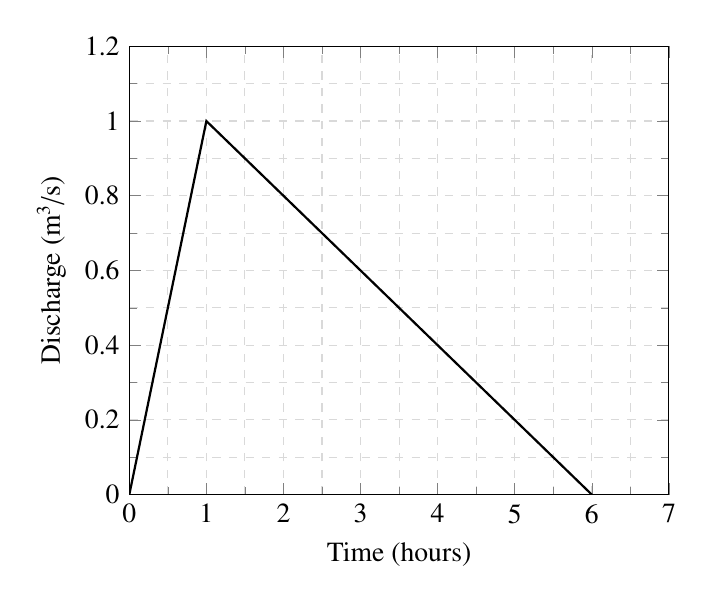
\begin{tikzpicture}
\begin{axis}[
    xlabel={Time (hours)},
    ylabel={Discharge (m$^3$/s)},
    xmin=0, xmax=7,
    ymin=0, ymax=1.2,
    xtick={0,1,2,3,4,5,6,7},
    ytick={0,0.2,0.4,0.6,0.8,1,1.2},
    grid=both,
    minor tick num=1,
    grid style={dashed,gray!30},
]

\addplot[
    color=black,
    thick,
    mark=none
] coordinates {
    (0,0) (1,1)  (6,0)
};

\end{axis}
\end{tikzpicture}

  % Use the correct path to your Q4.tex file
    \end{figure}
       



 
    \begin{enumerate}
        \item $\beta_1 > \beta_2$
        \item $\beta_1 < \beta_2$
        \item $\theta_1 > \theta_2$
        \item $\theta_1 < \theta_2$
    \end{enumerate}
    
    \item Which of the following statements about adverse yaw of an airplane is/are correct?
    \begin{enumerate}
        \item [P.] It is caused by flow separation resulting from large rudder deflection.
        \item [Q.]It is caused by dissimilar drag forces acting on the two halves of the wing resulting from aileron deflections of same magnitude.
        \item [R.]It can be eliminated by ensuring that the upward deflection of one aileron is greater than the downward deflection of the opposite aileron.
        \end{enumerate}
        \begin{enumerate}
           
        \item $P$ only
        \item $Q$ only
        \item $P$ and $R$
        \item $Q$ and $R$
    \end{enumerate}
    
    \item In a turbojet engine, the compressor outlet temperature increases with decreasing efficiency of the compressor. If the turbine inlet temperature remains constant, with decreasing efficiency of the compressor, the thrust specific fuel consumption of the engine
    \begin{enumerate}
        \item Decreases, as the heat input is lower.
        \item Remains unchanged.
        \item Increases, as the compressor needs more work input from the turbine.
        \item Decreases, as the thrust produced is higher.
    \end{enumerate}
    
    \item For a $1 m$ simply supported beam with a concentrated vertical load of 200 N and a concentrated bending moment of 100 Nm at the center as shown in the figure, the correct bending moment diagram is:

  \begin{figure}[H]
        \centering
        

    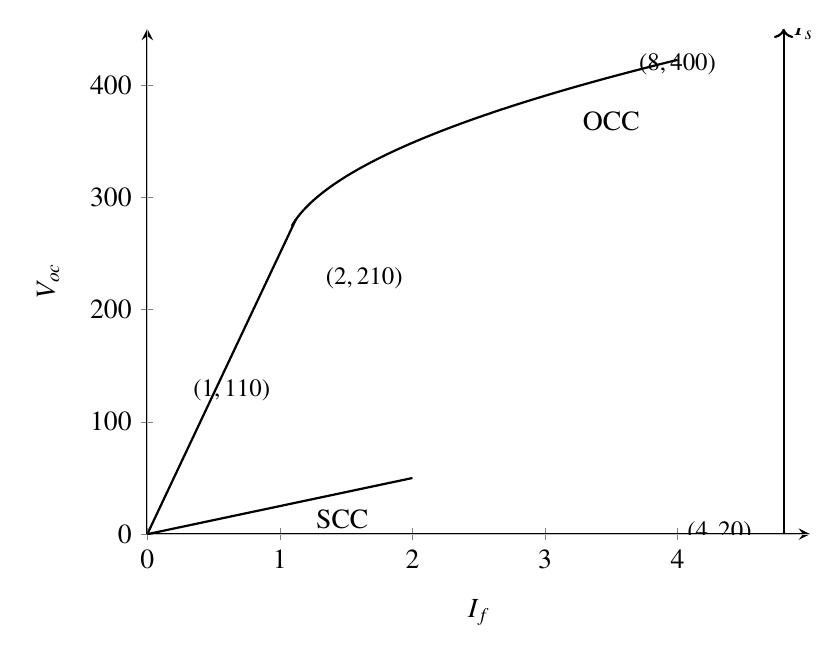
\begin{tikzpicture}
        \begin{axis}[
            axis lines = middle,
            xlabel = $I_f$,
            ylabel = $V_{oc}$,
            xmin = 0, xmax = 5,
            ymin = 0, ymax = 450,
            xtick = {0,1,2,3,4},
            ytick = {0,100,200,300,400},
            x label style={at={(axis description cs:1,0)},anchor=west},
            y label style={at={(axis description cs:0,1)},anchor=south},
            extra x ticks={0},
            extra y ticks={0},
            extra tick style={grid=major},
            axis line style=thick,
            xlabel near ticks,
            ylabel near ticks,
            every axis plot/.append style={thick},
            legend pos = north west,
            width=10cm, height=8cm,
        ]

        % Plot for OCC curve
        \addplot[domain=1.09:4, samples=100, smooth] {100*(x-1.03)^(0.5)+250};

        % Plot for SCC curves
        \addplot[domain=0:2, samples=2] {25*x};
        \addplot[domain=0:1.12, samples=2] {250*x};

        % Points with labels
        \node at (axis cs:0,0) [below left] {\small $(0,0)$};
        \node at (axis cs:0,10) [left] {\small $(0,10)$};
        \node at (axis cs:1,110) [above left] {\small $(1,110)$};
        \node at (axis cs:2,210) [above left] {\small $(2,210)$};
        \node at (axis cs:4,20) [below right] {\small $(4,20)$};
        \node at (axis cs:4,400) [above] {\small $(8,400)$};

        % Additional labels for OCC and SCC curves
        \node at (axis cs:3.5,350) [above] {OCC};
        \node at (axis cs:1.2,30) [below right] {SCC};

        % Right-hand axis line and label
        \draw[->, thick] (axis cs:4.8,0) -- (axis cs:4.8,450) node [right] {$I_{sc}$};

        % Top axis label for V_oc
        \node[above] at (axis cs:0,450) {$V_{oc}$};

        \end{axis}
    \end{tikzpicture}
   
  % Use the correct path to your Q4.tex file
    \end{figure}
    
    

    \item For real $x$, the number of points of intersection between the curves $y = x$ and $y = \cos x$ is {\underline{\hspace{1cm}}}.
   
    
    \item One of the eigenvalues of the following matrix 
    $\begin{bmatrix}
x & 2 \\
-1 & 3 \\
\end{bmatrix}$
is $1$. The other eigenvalue is {\underline{\hspace{1cm}}}.
    
    \item The curve $y = f(x)$ is such that its slope is equal to $y^2$ for all real $x$. If it passes through $(1, -1)$, the value of $y$ at $x = -2$ is {\underline{\hspace{1cm}}}.(round  off to 1 decimal place).
    

    \item The inviscid, incompressible flow field resulting from a uniform flow past a circular cylinder of radius $R$ centered at the origin is given by:\\
    $u_r=U(1-(\frac{R^2}{r^2}))\cos \theta$ \\      $u_r=-U(1+(\frac{R^2}{r^2}))\sin \theta$

    
  \begin{figure}[H]
        \centering
        
    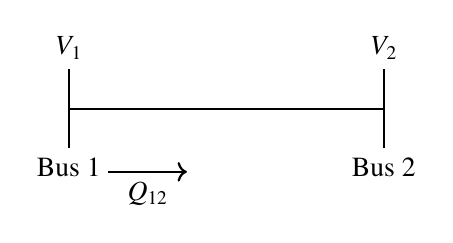
\begin{tikzpicture}
        % Draw the buses
        \draw[thick] (-2,0) -- (-2,1) node[above] {$V_1$};
        \draw[thick] (2,0) -- (2,1) node[above] {$V_2$};
        
        % Draw the line between the buses
        \draw[thick] (-2,0.5) -- (2,0.5);
        
        % Label the buses
        \node[below] at (-2,0) {Bus 1};
        \node[below] at (2,0) {Bus 2};
        
        % Draw the power flow arrow
        \draw[->, thick] (-1.5, -0.3) -- (-0.5, -0.3) node[midway, below] {$Q_{12}$};
    \end{tikzpicture}
     % Use the correct path to your Q4.tex file
    \end{figure}


    where $u_r$ and $u_\theta$ are the radial and azimuthal velocity components in polar coordinates,$(r,\theta)$,as shown in the figure.$U$ is the free stream speed.Ignore the effects of gravity.The azimuthal location (in the first quadrant) on the cylinder at which the pressure coefficient is zero is {\underline{\hspace{1cm}}} degrees(round off to the nearest integer).

    \item A cylindrical container of radius $R = 50 \, \text{cm}$ is filled with water up to a height $h_o$. Upon rotating the cylinder about its central axis at a constant angular speed, the free surface takes a parabolic shape (see figure),and is displaced upwards by $h_1 = 10 \, \text{cm}$ at $r = R$. The magnitude of the downward displacement $h_2$ of the free surface at $r = 0$ is {\underline{\hspace{1cm}}} cm (rounded off to the nearest integer).

        
  \begin{figure}[H]
        \centering
        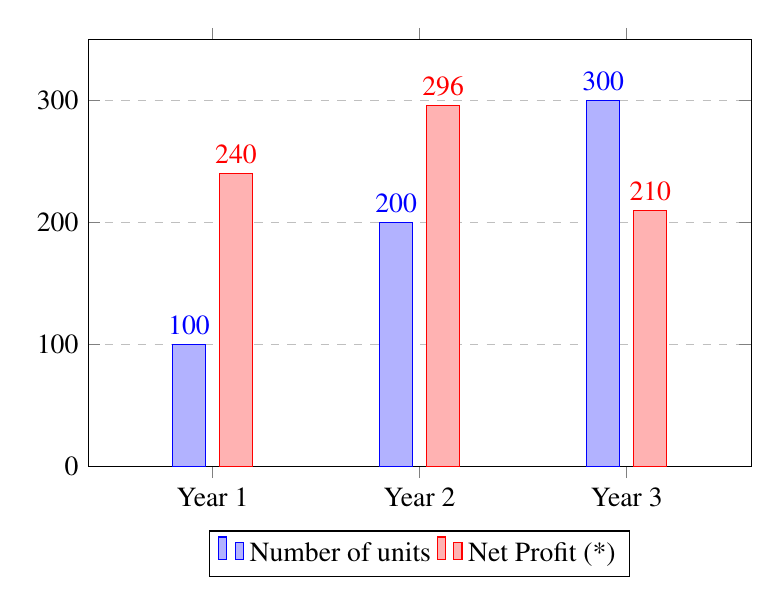
\begin{tikzpicture}
\begin{axis}[
    ybar=5pt,
    bar width=12pt,
    width=10cm, height=7cm,
    ymin=0, ymax=350,
    ylabel={},
    symbolic x coords={Year 1, Year 2, Year 3},
    xtick=data,
    nodes near coords,
    legend style={at={(0.5,-0.15)},anchor=north,legend columns=-1},
    enlarge x limits=0.3,
    ymajorgrids=true,
    grid style=dashed
]

\addplot coordinates {(Year 1, 100) (Year 2, 200) (Year 3, 300)};
\addplot coordinates {(Year 1, 240) (Year 2, 296) (Year 3, 210)};

\legend{Number of units, Net Profit (*)}

\end{axis}
\end{tikzpicture}  % Use the correct path to your Q4.tex file
    \end{figure}

    \item A two-dimensional, incompressible fluid flow described by the stream function $\psi = xy^3 m^2/s $ on the Cartesian plane. If the density and dynamic viscosity of the fluid are $1 \, \text{kg/m}^3$ and $0.1 \, \text{kg/m-s}$, respectively, the magnitude of the pressure gradient in the x-direction at $x = 1 \, \text{m}$ and $y = 1 \, \text{m}$ is {\underline{\hspace{1cm}}} $N/m^3$ (rounded off to 1 decimal place):
    

    \item The static pressure ratio across a stationary normal shock is given by 
    \[
\frac{P_2}{P_1} = 1+\frac {2\gamma}{\gamma+1}(M_1^2-1)
\]
    where $M_1$ is the upstream Mach number.For a stationary normal shock in air ($\gamma = 1.4, R = 287 \, \text{J/kg-K}$) with upstream flow conditions given by:speed $800m/s$, static  temperature $ 300 \, \text{K}$ and static pressure $1 \, \text{atm}$, the static pressure downstream of the shock is {\underline{\hspace{1cm}}} $\text{atm}$.(round off to 2 decimal places).


    
    \item For a symmetric airfoil at an angle of attack of $10^\circ$, assuming thin airfoil theory, the magnitude of the pitching moment coefficient about the leading edge is {\underline{\hspace{1cm}}}(round off to 2 decimal places).
    

    \item The span-wise distribution of circulation over a finite wing of span $b = 10 \, \text{m}$ is 
    \[
    \Gamma(y) = \Gamma_0 \sqrt{1 - (\frac{2y}{b})^2}
    \]
    If $\Gamma_0 = 20m^2/s$ and the free stream density and speed are $1.2 \, \text{kg/m}^3$ and $100 \, \text{m/s}$, respectively, the total lift is {\underline{\hspace{1cm}}} kN (round off to 2 decimal places).
   










\end{enumerate}
\end{document}